\section{Heavy-tailed Distribution And Light-tailed Distribution}	

	\frame{
	\begin{center}
{\tnewroman \textbf{\Huge{Heavy-tailed Distribution And Light-tailed Distribution}}}
	\end{center}	
}
\begin{frame}

\frametitle{承前启后}
\qquad 如果捕食者像无头苍蝇一样漫无目的的做布朗运动,真的能很有效的地寻到到猎物吗?在数学上可以证明,布朗运动和分子自由扩散一样,单位速度的分子在时间$t$内平均只有$\sqrt{t}$的位移量。若捕食者采用这种策略,需要很久才能够成功。

\qquad 那么有没有比布朗运动更高效的搜索方法呢?一组巴西物理学家于$1999$年提出了一个设想,认为“莱维飞行”比布朗运动有更高的搜索效率,因此自然会偏向与采用“莱维飞行”捕食的生物。为了理解什么是“莱维飞行”,我们首先需要对概率分布的轻尾性和重尾性有一个认识。
%\tableofcontents

\end{frame}
	
\begin{frame}
\frametitle{指数分布}
指数分布是描述泊松过程中的事件之间的时间的概率分布,即事件以恒定平均速率连续且独立地发生地过程。它是几何分布的
连续模拟,它具有无记忆的关键性质。例如,如果T是某一元件的寿命,已知元件使用了$t$小时,它总共使用至少$s+t$小时的条件概率与一开始使用时算起它使用至少s小时的概率相等。

其概率密度函数:

\begin{displaymath}
F\left ( x;\lambda  \right )= \left\{\begin{matrix}
1-e^{-\lambda x}, &x\geq 0  \\
0, &x< 0
\end{matrix}\right.
\end{displaymath}

\end{frame}

\begin{frame}
\frametitle{轻尾分布}
\qquad 比指数分布尾部更薄的概率分布是轻尾分布。 它们下降到$0$的速度比指数分布的速度快得多,因此在尾部质量更小。 Gumbel 分布是轻尾分布的一个例子。轻尾分布并不能很好地反映“真实世界”的数据。



\centering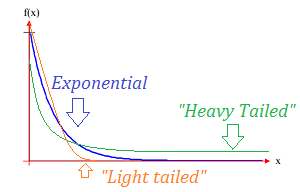
\includegraphics[scale=0.5]{images/light-tailed.png}


\end{frame}

\begin{frame}

\frametitle{概率分布的轻尾性}
\qquad 前面说过,布朗运动的步长服从正态分布。正态分布是一种典型的{\color{red}{轻尾分布}}, 也就是说,不太可能取得极端值的分布。

\begin{figure}
	\centering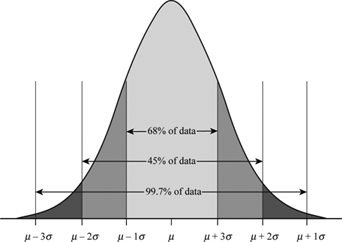
\includegraphics[scale=0.35]{images/normal_distribution.png}
\end{figure}

表达式$y= \frac{1}{\sqrt{2\pi}\sigma}e^{\frac{-\left ( x-\mu  \right )^{2}}{2\sigma ^{2}}}$。其中$\mu$是均值,$\sigma$是标准差。当$x$增大
时,函数下滑趋势非常快,因此数学家又将正态分布函数纳入速降函数空间范畴。速降函数是专门为傅里叶分析而量身定做的。
%\begin{definition}
%    definition 1...
%\end{definition}

\end{frame}

\begin{frame}

\frametitle{概率分布的重尾性}
\qquad 而在现实生活中,大多数的事情不能用轻尾分布来描述,例如保险领域的保险金-事故可以看作是稀有事件,但一旦发生并通过审核,保险公司就必须大量金额,这样一来保险金的分布就很可能取到很大的值。为了描述这样容易取得极值的随机变量,我们需要引入重尾分布。

\centering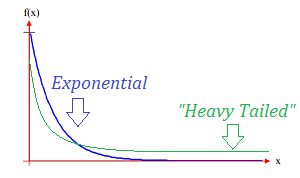
\includegraphics[scale=0.5]{images/heavy_tailed.png}

典型特点: 大头短$+$小尾长。“莱维飞行”的平均位移是$t^{\gamma}$,$\gamma>\frac{1}{2}$.
\end{frame}
\begin{frame}
\frametitle{重尾分布}
当$x\rightarrow \infty$时,重尾分布下降到$0$的速度慢于指数分布。因而尾部质量较大。其数学定义为:

\begin{displaymath}
\lim_{x\rightarrow \infty }e^{\lambda x}F\left ( x \right )=\infty
\end{displaymath}

其中,$\lambda>0$, $F(x)$是尾分布函数。

重尾分布更适用于对那些离峰值较远的稀有事件也会有相当的概率发生的情况。重尾分布作为一个大的类别,还包含三个重要的子类别,分别是肥尾分布(Fat-tailed distribution),长尾分布(Long-tailed distribution)和次指数分布(Subexponential distribution)
\end{frame}

\begin{frame}

\frametitle{概率分布的重尾性}
\qquad 那么,如何验证“莱维飞行”的有效性呢?一个方案就是前面提到的大肠杆菌的{\color{red}{趋化行为}}。尽管最初的“莱维飞行”假说是针对动物
而言的,但从大肠杆菌的游击战策略可以看出,该假说对微生物同样适用!这样一来,对微生物的研究也能反过来帮助人们更深入地理解动物行为,这便是微观的细胞生物学在宏观的生态学中的应用。

\end{frame}

\begin{frame}
\frametitle{莱维过程}
\qquad 莱维过程$\left \{ X\left ( t \right ),t\geq 0 \right \}$是一种随机过程,它满足的条件比布朗运动宽松:
\begin{itemize}
\item $X{0}$ 几乎处处为0;
\item 独立增量性;
\item 稳定增量性;
\item 样本轨道右连续.
\end{itemize}


\qquad 连续的布朗运动和离散的泊松过程都是莱维过程的特例。因此可以大胆猜测,莱维过程就是带“跳跃”的布朗运动。正是这些不连续
性的“跳跃”给予莱维过程“重尾”的特性。
\end{frame}